\documentclass[../main]{subfiles}
\newcommand*\circled[1]{\tikz[baseline=(char.base)]{
            \node[shape=circle,draw,inner sep=1pt] (char) {#1};}}
    \begin{document}
    \setcounter{secnumdepth}{2}
    \chapter{提案手法}
        \section{提案手法の概要}
        本研究は,全天球カメラから取得した画像に基づき通路の特徴を分類する手法を提案する.
        また,本研究では先行研究と同様の8種類の通路の特徴を分類する.

        
        本手法の通路分類の流れを\fref{figure::proposed_method}に示す.
        まず,全天球カメラで水平360度の画像データを収集する.次に,YOLOの学習器を用いて画像中の通路やドアなどの物体を検出する.
        通路が検出された場合,通路が検出された方向からどの通路の特徴に相当するかを分類する.
        \fref{figure::proposed_method}の例では,学習器の出力結果から通路が3つ検出されている.また,通路はカメラを取り付けたロボットに対して前,後ろ,
        右方向に検出されている.この通路の特徴から,通路は右に曲がれる三叉路に分類される.
        
        %提案手法の簡単な例
        \begin{figure}[H]
            \centering
            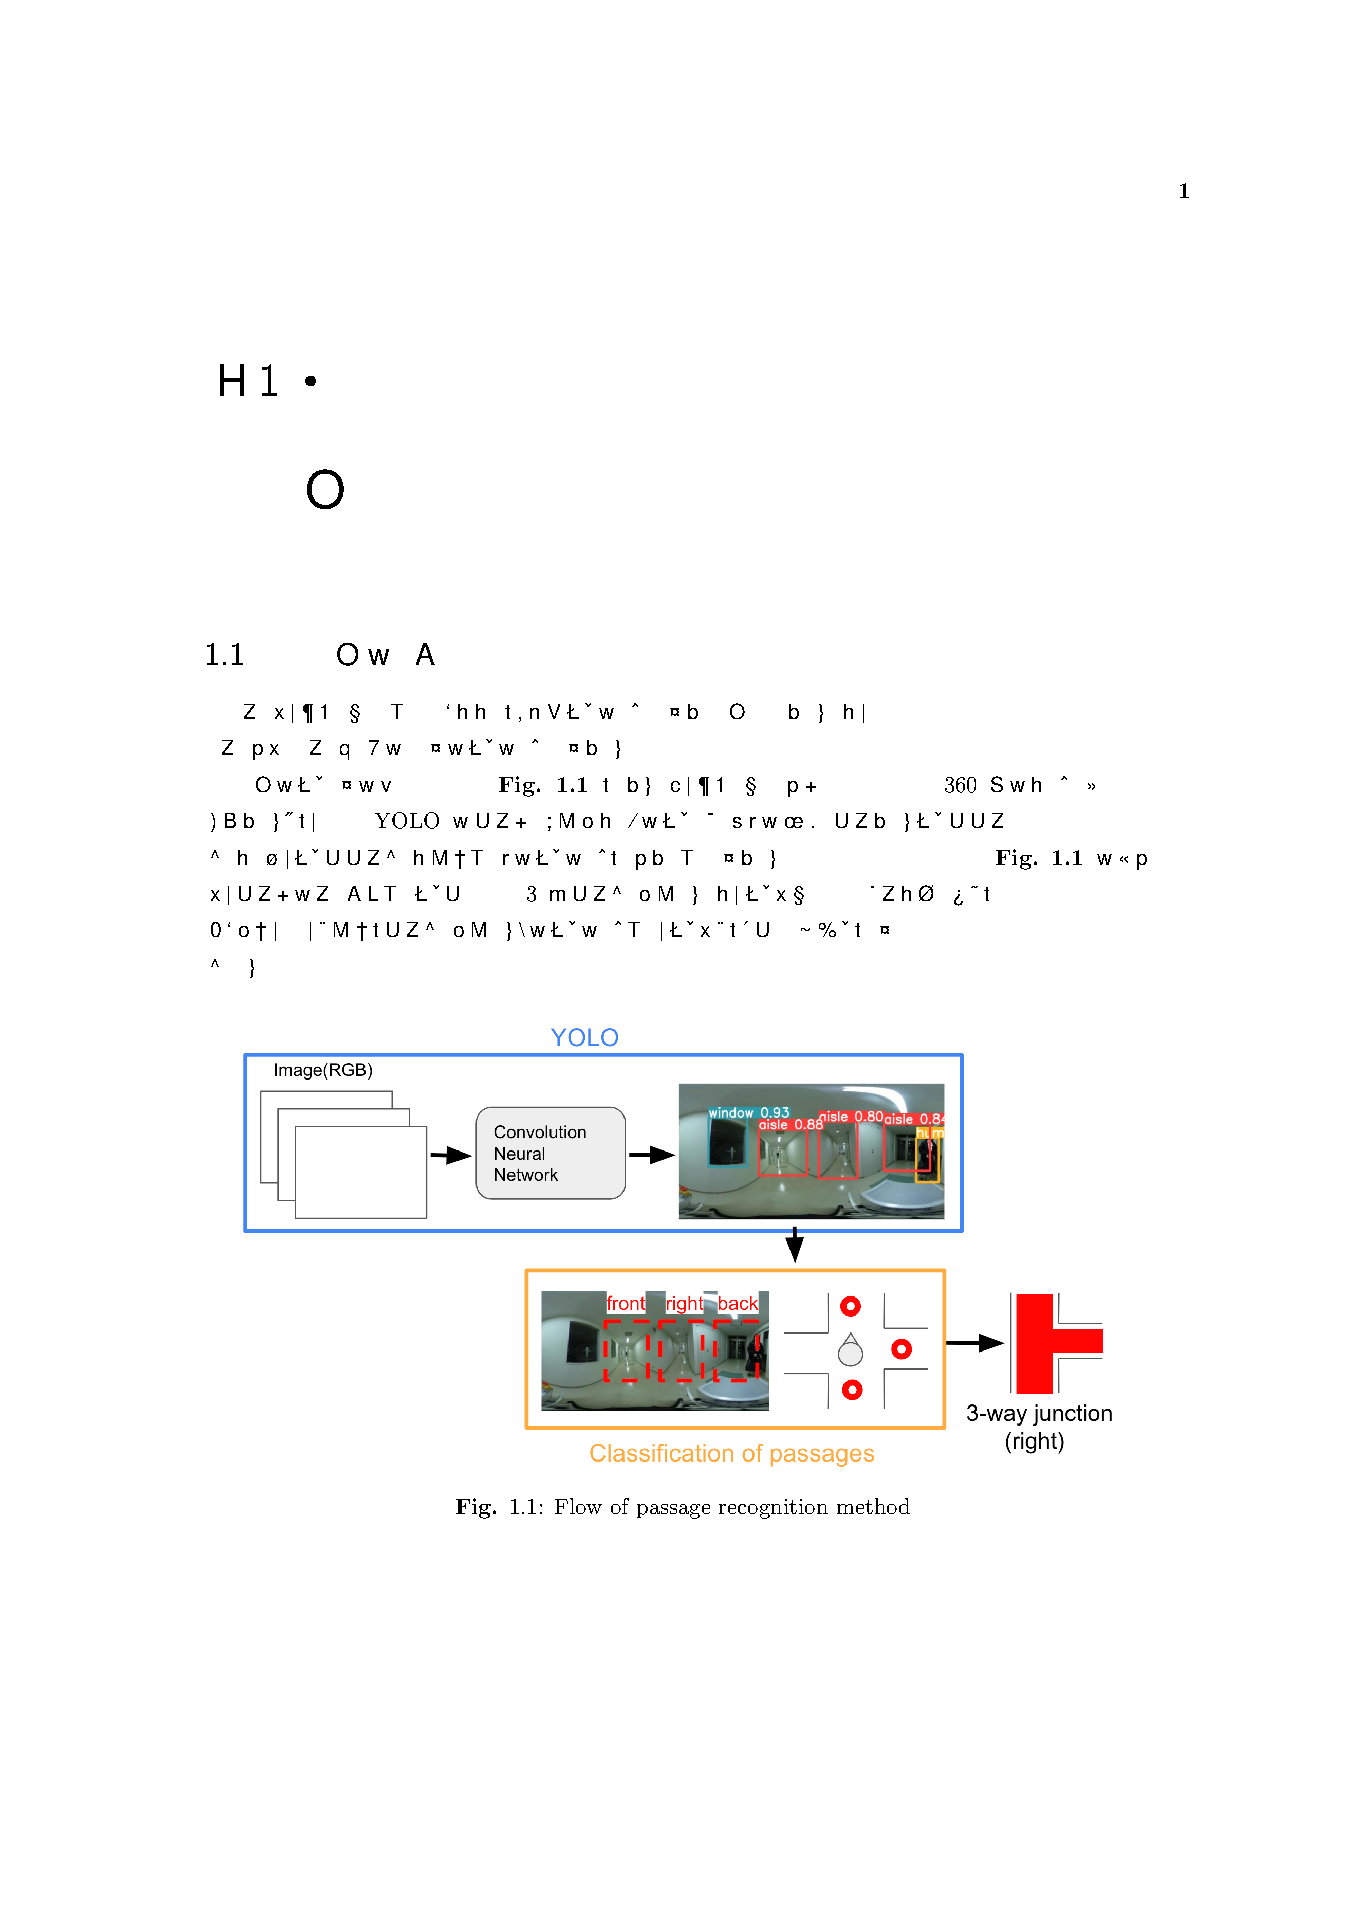
\includegraphics[width=15cm]{../images/proposed_method.png}
            \caption{Flow of passage recognition method}
            \label{figure::proposed_method}
        \end{figure}

        \newpage

        \section{データセットの作成}
        学習モデル作成のため,独自に作成した通路の画像を集めたデータセットを用いて学習を行う.
        学習に用いる画像は千葉工業大学津田沼キャンパス2号館3階の廊下で収集した.
        全天球カメラで取得した画像は通常,\fref{subfigure::no_proc}に示すようにカメラの正面にくる物体が画像の中心に写り,
        後方の物体は画像の左端と右端で分割されてしまう.
        本手法ではカメラの前後左右の各方向にある物体を正しく検出する必要があるため,後方の物体が分割されないようにデータセットの画像に対して
        \fref{subfigure::preproc}に示すような前処理を行う.この処理では,画像の左端1/8を切り取り,右端にスライドさせるという内容の処理を行う.


        データセットは合計3554枚の画像により構成されており,その一部を\fref{figure::dataset_fig}に示す.
        また,データセットのクラスは\fref{table::datasets_table}に示す11クラスとした.
        作成したデータセットで人をラベル付した理由は,実験中にロボットの後ろをついて歩く際,距離を取っている場合でも
        細い通路などで人が通路と被ることがあり,検出結果に支障をきたさないようにするためである.
        
    
        %画像の前処理の例
        % \begin{figure}[htbp]
        %   \centering
        %    \subfigure[no processing image]{\includegraphics[height=4cm]{../images/no_processing.png}
        %    \label{subfigure::no_proc}}
        %    \subfigure[preprocessing image]{\includegraphics[height=4cm]{../images/after_processing.png}
        %    \label{subfigure::preproc}}
        %    \caption{Preprocessing of spherical camera images}
        %    \label{figure::proc_exp}
        % \end{figure}
        
        \begin{figure}[htbp]
            \centering
            \begin{tabular}{cc}
              %---- 最初の図 ---------------------------
              \begin{minipage}[c]{\textwidth}
                \centering
                \includegraphics[height=4cm]{../images/no_processing.png}
                \subcaption{no processing image}
                \label{label::no_proc}
              \end{minipage}\\
              %\hspace*{1cm}
              %---- 2番目の図 --------------------------
              \begin{minipage}[c]{\textwidth}
                \centering
                \includegraphics[height=4cm]{../images/proc_image2.png}
                \subcaption{Preprocessing images}
                \label{label::proc_exp}
              \end{minipage}
              %---- 図はここまで ----------------------
            \end{tabular}
            \caption{Preprocessing of spherical camera images}
        \end{figure}

        %自作データセットの画像例
        \begin{figure}[H]
         \centering
         \includegraphics[width=16cm]{../images/dataset_exp.png}
         \caption{An example of a dataset}
         \label{figure::dataset_fig}
        \end{figure}

        %データセットのクラス数
        \begin{table}[H]
            \caption{Class name to be labeled}
            \centering
            \label{table::datasets_table}
            \begin{tabular}{lllll}
            \hline
            name of the class &  &  &  &  \\ 
            \hline \hline
            aisle             &  &  &  &  \\
            end               &  &  &  &  \\
            door\_end         &  &  &  &  \\
            human             &  &  &  &  \\
            door              &  &  &  &  \\
            step              &  &  &  &  \\
            square            &  &  &  &  \\
            vending\_machine  &  &  &  &  \\
            trash\_can        &  &  &  &  \\
            signboard         &  &  &  &  \\
            window            &  &  &  &  \\ 
            \hline
            \end{tabular}
        \end{table}            

        \section{学習の結果}
        作成したデータセットを用いてYOLOv5により学習を行う.トレーニングに用いたネットワークを\fref{figure::}に示す.
        また,学習に用いるデータの構成とハイパーパラメータの設定を\fref{table::learning}に示す.
        

        学習の結果,作成したモデルの精度は0.95であった.
        また,学習中のLossの推移は\fref{figure::training_loss}のようになり,過学習が起きていないことが確認できる.

        \begin{table}[H]
            \caption{Structure of data used for learning}
            \centering
            \label{table::learning}
            \begin{tabular}{l|l}
            \hline
            \multicolumn{1}{c|}{training}   & \multicolumn{1}{c}{3540}                \\ \hline
            \multicolumn{1}{c|}{validation} & \multicolumn{1}{c}{14}                  \\ \hline
            \multicolumn{1}{c|}{epoch}      & \multicolumn{1}{c}{300}                \\ \hline
            \multicolumn{1}{c|}{batch}      & \multicolumn{1}{c}{8}                   \\ \hline
            \end{tabular}
        \end{table}

        \newpage

        \section{通路分類の手法}
        学習器により出力された物体検出の結果から,通路の特徴を分類する手法について述べる.
        作成した学習器による物体検出の結果を\fref{figure::detected_image}に示す.
        また,カメラに対する前後左右の各方向と,それに対応する画像の領域を\fref{figure::aisle_classification1}の赤枠により表す.
        本手法では,学習器により通路が検出された場合,検出された各通路のバウンディングボックスの中心座標を計算する.
        そして,中心座標が\fref{figure::aisle_classification1}の各赤枠の領域内にある場合,対応する方向に通路があるとして扱う.
        最終的に,\tref{table::aisle_type}に示すように,通路がある方向から画像の通路がどの通路の特徴に相当するのかを分類する.

        \begin{figure}[htbp]
            \centering
            \begin{tabular}{cc}
              %---- 最初の図 ---------------------------
              \begin{minipage}[c]{\textwidth}
                \centering
                \includegraphics[width=13cm]{../images/yolo_aisle.jpg}
                \subcaption{Output result of object detection by learner}
                \label{figure::detected_object}
              \end{minipage}\\
              %---- 2番目の図 --------------------------
              \begin{minipage}[c]{\textwidth}
                \centering
                \includegraphics[width=13cm]{../images/aisle_classification1.png}
                \subcaption{Positional relationship between the area in the image and each direction with respect to the camera}
                \label{figure::aisle_classification1}
              \end{minipage}
              %---- 図はここまで ----------------------
            \end{tabular}
        \end{figure}





\end{document}